\documentclass[12pt,a4paper,hidelinks]{article}
\usepackage[english,italian]{babel}
\usepackage{float}
\usepackage{amsmath, amssymb, pifont, geometry, tikz, hyperref, newlfont, graphicx, caption, array, multirow, tabularx, svg, pdfpages}
\usepackage{listings}
\renewcommand{\lstlistingname}{Listato}
\usepackage{xcolor}
\usepackage{setspace}
\usepackage{csquotes}
\usepackage[
backend=biber,
style=numeric,
sorting=ynt
]{biblatex}
\addbibresource{bibliography.bib}
\usepackage{pgf-pie}
\usepackage{longtable}
\usepackage[T1]{fontenc}
\usepackage[utf8]{inputenc}
\usepackage{booktabs}
\usepackage{pgfplots}
\usepackage{amsmath}
\usepackage{caption}
\pgfplotsset{compat=1.17}
\usepgfplotslibrary{statistics}

\definecolor{logc}{HTML}{55A868}
\definecolor{prec}{HTML}{4C72B0}
\definecolor{postc}{HTML}{DD8452}
\definecolor{sigc}{HTML}{C44E52}

\hypersetup{
bookmarksopen=true,	
pdfauthor=Matteo Lublanis
}

\lstdefinestyle{myStyle}{
  language=SQL,
  basicstyle=\small\ttfamily,
  keepspaces=true
}

\lstdefinestyle{myStyle2}{
  language=SQL,
  basicstyle=\small\ttfamily,
  keepspaces=true,
  numbers = left,
  numbersep=1pt
}

\definecolor{codegreen}{rgb}{0,0.6,0}
\definecolor{codegray}{rgb}{0.5,0.5,0.5}
\definecolor{codepurple}{rgb}{0.58,0,0.82}
\definecolor{backcolour}{rgb}{0.95,0.95,0.92}

\lstdefinestyle{myStyle3}{
    language=SQL,
    backgroundcolor=\color{backcolour},   
    commentstyle=\color{codegreen},
    keywordstyle=\color{magenta},
    numberstyle=\tiny\color{codegray},
    stringstyle=\color{codepurple},
    basicstyle=\ttfamily\footnotesize,
    breakatwhitespace=false,         
    breaklines=true,                 
    captionpos=b,                    
    keepspaces=true,                 
    numbers=left,                    
    numbersep=5pt,                  
    showspaces=false,                
    showstringspaces=false,
    showtabs=false,                  
    tabsize=2
}

\lstdefinestyle{py}{
    language=Python,
    backgroundcolor=\color{backcolour},   
    commentstyle=\color{codegreen},
    keywordstyle=\color{magenta},
    numberstyle=\tiny\color{codegray},
    stringstyle=\color{codepurple},
    basicstyle=\ttfamily\footnotesize,
    breakatwhitespace=false,         
    breaklines=true,                 
    captionpos=b,                    
    keepspaces=true,                 
    numbers=left,                    
    numbersep=5pt,                  
    showspaces=false,                
    showstringspaces=false,
    showtabs=false,                  
    tabsize=2
}

\graphicspath{{figures/}}

\newcommand{\tabellaValutazioneEuristica}[6]{
	\noindent
	\begin{tabularx}{\textwidth}{|X|}
		\hline
		\begin{minipage}[t]{\linewidth}\raggedright
			\vspace{4pt}
			\textbf{Problema N\textsuperscript{o}:} #1 \hfill \textbf{Grado di Severità:} #5\\[4pt]
			\textbf{Posizione:} #2\\[6pt]
			\textbf{Descrizione:} \par
			#3\\[6pt]
			\textbf{Principi Violati:} \par
			#4
			\vspace{6pt}
		\end{minipage} \\ \hline
		
		\begin{minipage}[t]{\linewidth}\centering
			\vspace{4pt}
			\textbf{Screenshot:}
			\vspace{0.6em}
			
			#6
			\vspace{6pt}
		\end{minipage} \\ \hline
	\end{tabularx}
	\vspace{1em}
}

\newcommand{\tabellaMockup}[6]{
	\noindent
	\begin{tabularx}{\textwidth}{|X|}
		\hline
		\begin{minipage}[t]{\linewidth}\raggedright
			\vspace{4pt}
			\textbf{Numero:} #1\\[6pt] 
			\textbf{Posizione:} \par 
			#2\\[6pt]
			\textbf{Problema/i Risolto/i:} \par
			#3\\[6pt]
			\textbf{Descrizione:} \par
			#4\\[6pt]
			\textbf{Pattern Adottato/i:} \par
			#5
			\vspace{6pt}
		\end{minipage} \\ \hline
		
		\begin{minipage}[t]{\linewidth}\centering
			\vspace{4pt}
			\textbf{Screenshot del Mockup:}
			\vspace{0.6em}
			
			#6
			\vspace{6pt}
		\end{minipage} \\ \hline
	\end{tabularx}
	\vspace{1em}
}
\textwidth=450pt\oddsidemargin=0pt
\begin{document}

\begin{titlepage}
	\begin{center}
		\begin{spacing}{1.5}
			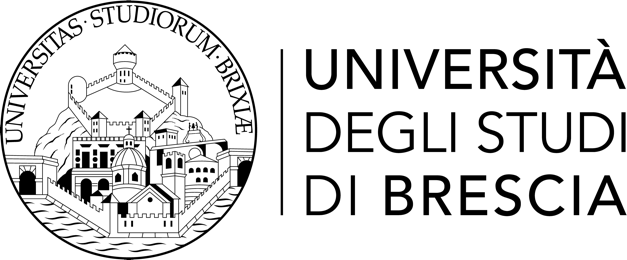
\includegraphics[width=0.6\textwidth]{figures/frontespizio.png}\\
			{\Large \textsc{Dipartimento di Ingegneria dell'Informazione}}\\
			{\large \it Corso di Laurea in Ingegneria Informatica}
		\end{spacing}
	\end{center}
	
	\vspace{15mm}
	
	\begin{center}
		\begin{spacing}{1.5}
			{\large Relazione del corso di Interazione Persona-Calcolatore}
			
			{\LARGE \textsc{Riprogettazione di un'applicazione web bancaria}}
		\end{spacing}
	\end{center}
	
	\vspace{35mm}
	
	\noindent
	\begin{minipage}[t]{0.50\textwidth}
		{\large \textbf{Professoressa:}\\
			Daniela Fogli}
	\end{minipage}
	\hfill
	\begin{minipage}[t]{0.50\textwidth}
		\begin{flushleft}
			{\large \textbf{Componenti:}\\
				Singh Sahiljit (Matr.~740552)\\
				Lublanis Matteo (Matr.~736418)}
		\end{flushleft}
	\end{minipage} 
	
	\vspace{25mm}
	
	\begin{center}
		{\large \it Anno Accademico 2025/2026}
	\end{center}
\end{titlepage}


\tableofcontents

% inserisci i file contenenti le sezioni

\section{Descrizione del Sistema}

L'applicazione presa in esame in questo progetto è una \textbf{web application bancaria} che fornisce funzionalità di home banking e gestione dei servizi bancari di base. L'applicazione si propone di coprire tre principali aree di utilizzo, ciascuna destinata a una specifica categoria di utenti:

\subsection{Categorie di Utenti}

\subsubsection{Clienti}
I clienti della banca possono accedere a un'interfaccia intuitiva per gestire le principali operazioni bancarie online, come:
\begin{itemize}
	\item Visualizzazione del saldo e della lista movimenti;
	\item Bonifici e trasferimenti di denaro;
	\item Gestione dei propri dati anagrafici.
\end{itemize}

\subsubsection{Employee}
I dipendenti della banca possono accedere a un pannello dedicato che consente di:
\begin{itemize}
	\item Visualizzare e modificare i dati dei clienti;
	\item Gestire operazioni richieste dai clienti in filiale;
	\item Gestire le credenziali per l'accesso dei clienti.
\end{itemize}

\subsubsection{Admin}
Gli admin hanno accesso completo alla gestione dell'utenza e delle funzionalità del sistema, con la possibilità di:
\begin{itemize}
	\item Creare, modificare e cancellare account (clienti e employee);
	\item Gestire le assegnazioni fra clienti e employee;
	\item Monitorare le attività del sistema.
\end{itemize}

\newpage 

\subsection{Principali Schermate dell'Applicazione}
\subsubsection{Schermate utente ancora non autenticato}

La Homepage presenta un bottone in alto a sinistra che permette all'utente di accedere. 

\begin{figure}[htbp]
	\centering
	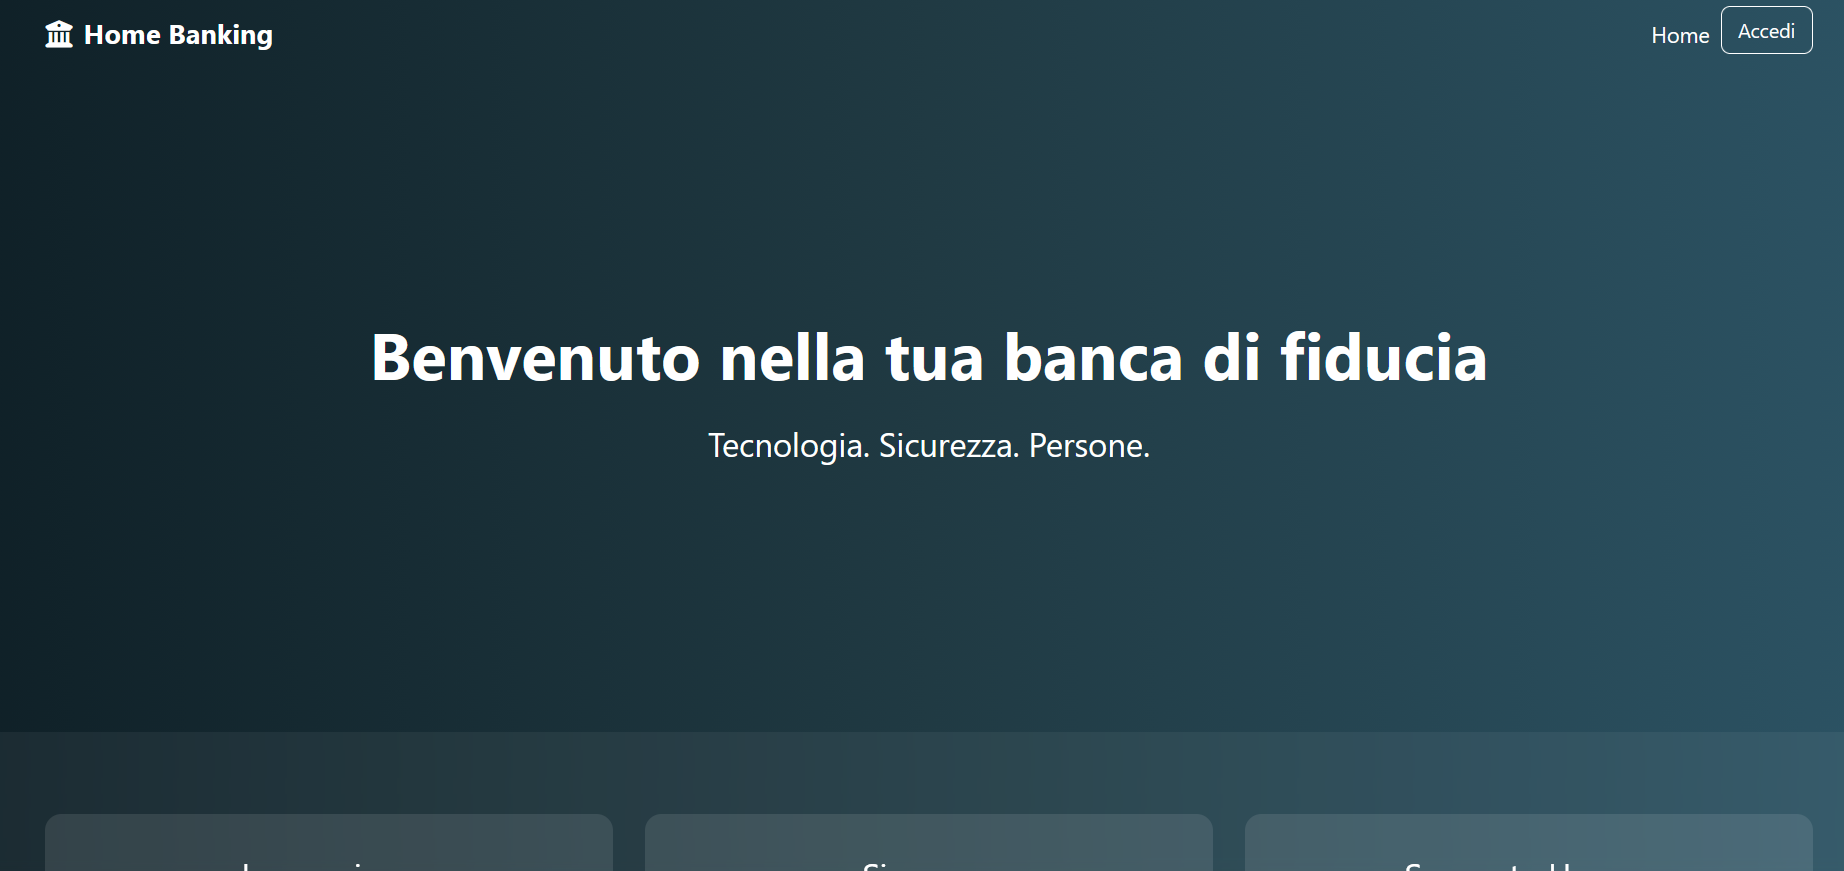
\includegraphics[width=0.8\textwidth]{schermata_principale}
	\caption{Homepage}
	\label{fig:schermata_principale}
\end{figure}

Una volta cliccato il bottone di login, l'utente vedrà due opzioni:
\begin{itemize}
	\item Accesso come cliente;
	\item Accesso come lavoratore (ovvero come employee oppure admin);
\end{itemize} 

\begin{figure}[htbp]
	\centering
	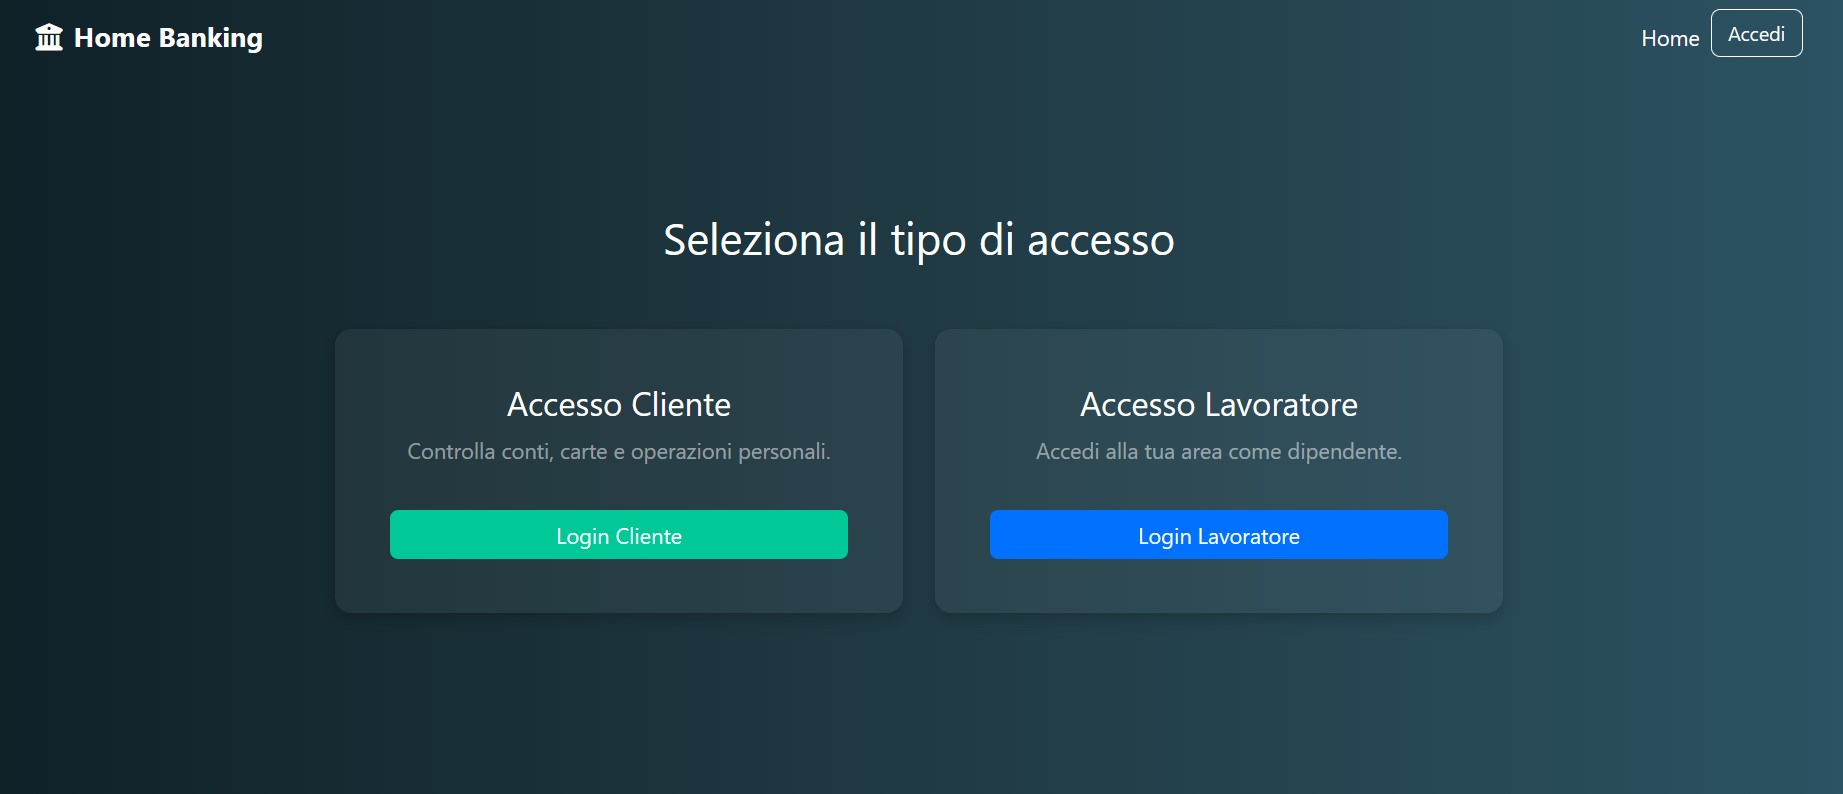
\includegraphics[width=0.8\textwidth]{selezione_tipologia_accesso}
	\caption{Schermata per selezionare la tipologia di accesso}
	\label{fig:selezione_tipologia_accesso}
\end{figure}

\clearpage

Nella pagina di login l'utente potrà inserire username e password. 

\begin{figure}[htbp]
	\centering
	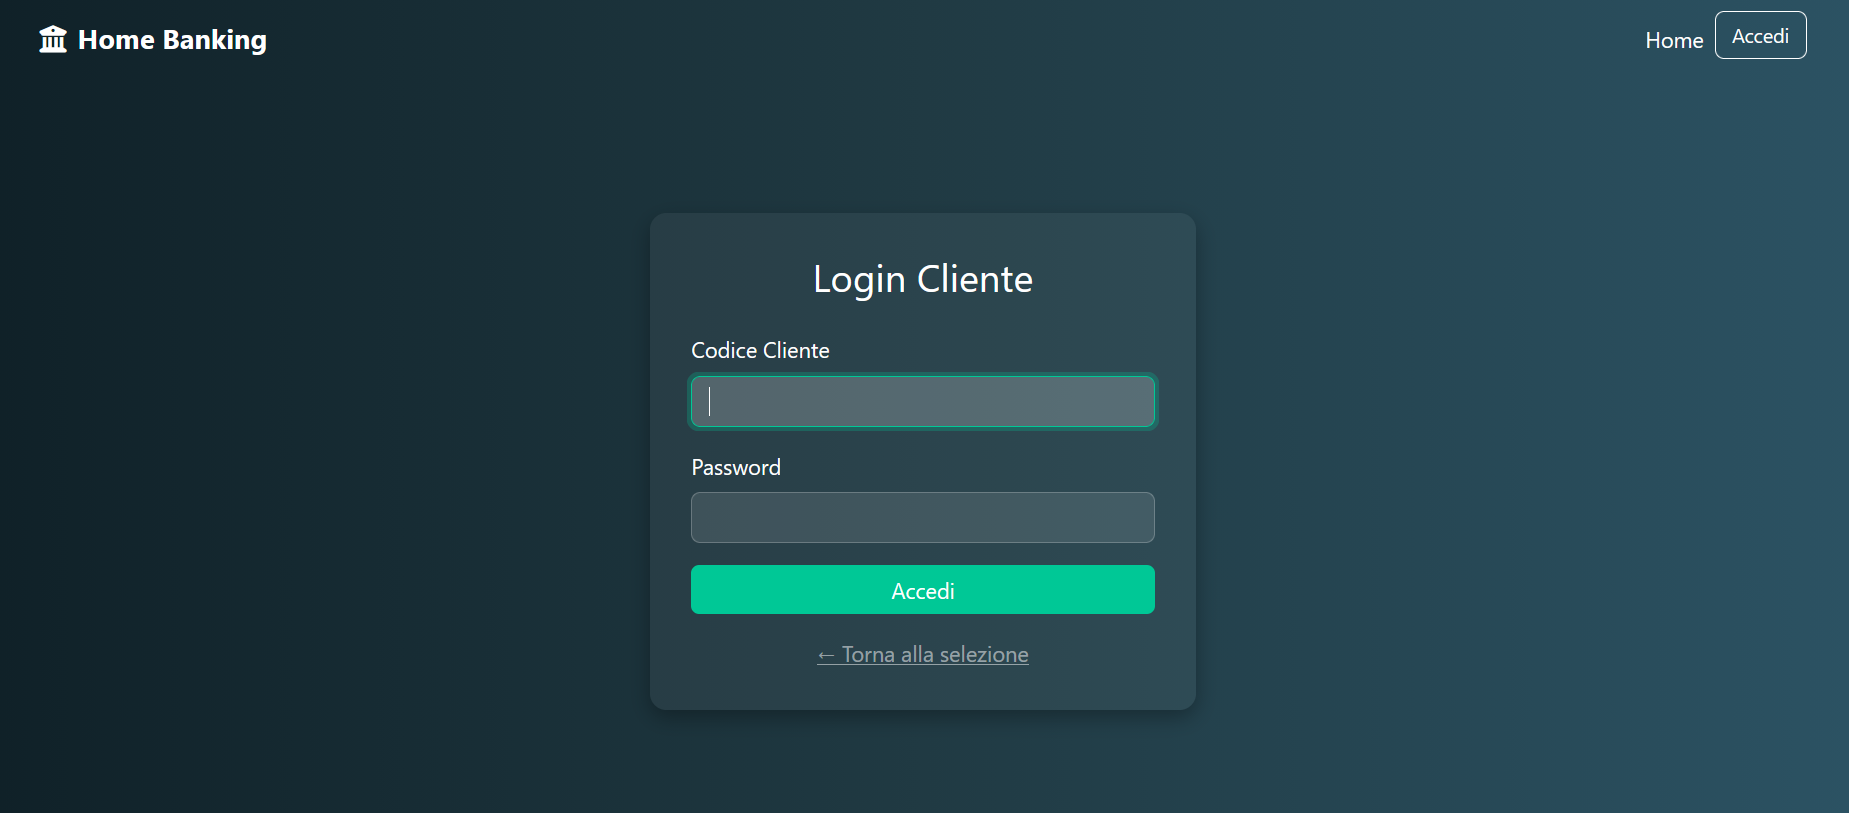
\includegraphics[width=0.8\textwidth]{login_cliente}
	\caption{Schermata login}
	\label{fig:login_cliente}
\end{figure}

\begin{figure}[htbp]
	\centering
	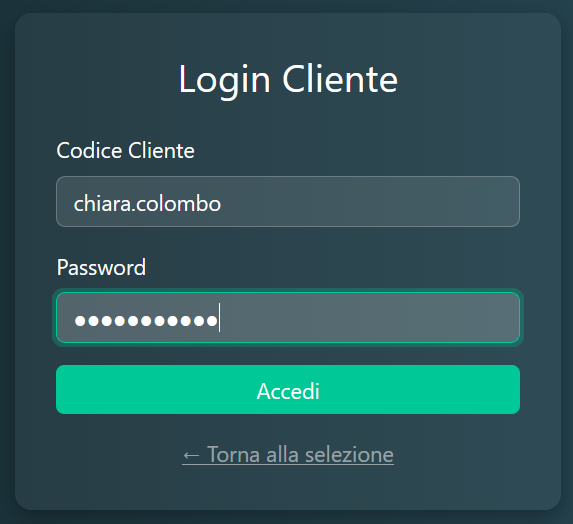
\includegraphics[width=0.5\textwidth]{login_compilato_cliente}
	\caption{Schermata login compilata}
	\label{fig:login_compilato_cliente}
\end{figure}

\section{Profili utente e Personas}
In questo capitolo verranno descritte le diverse tipologie di utenti che interagiranno con l’applicazione. L’analisi dei profili utente costituirà una base fondamentale per le fasi successive del progetto, in particolare per la valutazione euristica e per le attività di riprogettazione dell’interfaccia.
\\
\\
Come detto prima le tipologie di utente sono 3: Admin, Employee e Cliente

\subsection{Admin}
L'admin è colui che può utilizzare l'applicazione per eseguire qualsiasi tipo di procedura in quanto possiede i permessi più alti. 

\subsubsection{Caratteristiche psicologiche}
\begin{table}[h]
	\centering
	\begin{tabular}{|c|c|}
		\hline
		\textbf{Caratteristica} & \textbf{Tipologia} \\
		\hline
		Stile cognitivo & Analitico, verbale, astratto\\
		\hline
		Attitudine & Neutrale \\
		\hline
		Motivazione & Alta \\
		\hline
	\end{tabular}
	\caption{Caratteristiche psicologiche dell'admin}
\end{table}

\subsubsection{Caratteristiche di conoscenza}
\begin{table}[h]
	\centering
	\begin{tabular}{|c|c|}
		\hline
		\textbf{Caratteristica} & \textbf{Tipologia} \\
		\hline
		Livello di alfabetizzazione & Buon livello \\
		\hline
		Titolo di studio & Laurea \\
		\hline
		Abilità dattilografica & Alta \\
		\hline
		Linguaggio nativo & Italiano \\
		\hline
		Alfabetizzazione informatica & Alta \\
		\hline
	\end{tabular}
	\caption{Caratteristiche di conoscenza dell'admin}
\end{table}

\clearpage
\subsubsection{Caratteristiche di esperienza}
\begin{table}[h]
	\centering
	\begin{tabular}{|c|c|}
		\hline
		\textbf{Caratteristica} & \textbf{Tipologia} \\
		\hline
		Esperienza del compito & Esperto \\
		\hline
		Esperienza sulla applicazione & Medio \\
		\hline
		Esperienza dei sistemi informatici & Media \\
		\hline
		Uso di altri sistemi & Scarso \\
		\hline
	\end{tabular}
	\caption{Caratteristiche di esperienza dell'admin}
\end{table}

\subsubsection{Caratteristiche fisiche}
\begin{table}[h]
	\centering
	\begin{tabular}{|c|c|}
		\hline
		\textbf{Caratteristica} & \textbf{Tipologia} \\
		\hline
		Daltonismo & Sì/No \\
		\hline
		Manualità & Variabile \\
		\hline
		Disabilità & Sì/No\\
		\hline
	\end{tabular}
	\caption{Caratteristiche fisiche dell'admin}
\end{table}

\subsubsection{Caratteristiche del lavoro e dei compiti}
\begin{table}[h]
	\centering
	\begin{tabular}{|c|c|}
		\hline
		\textbf{Caratteristica} & \textbf{Tipologia} \\
		\hline
		Uso sistema & Obbligatorio \\
		\hline
		Frequenza d'uso & Media \\
		\hline
		Addestramento di base & Obbligatorio formale \\
		\hline
		Categorie di lavoro & Manager \\
		\hline
		Uso di altri strumenti & No \\
		\hline
		Frequenza del turnover & Basso \\
		\hline
		Importanza del compito & Alto \\
		\hline
		Struttura del compito & Media \\
		\hline
	\end{tabular}
	\caption{Caratteristiche del lavoro e dei compiti dell'admin}
\end{table}

\clearpage
\subsection{Employee}
L'employee è colui che lavora per la banca allo sportello. Può svolgere svariati compiti poiché possiede un livello medio di permessi.

\subsubsection{Caratteristiche psicologiche}
\begin{table}[h]
	\centering
	\begin{tabular}{|c|c|}
		\hline
		\textbf{Caratteristica} & \textbf{Tipologia} \\
		\hline
		Stile cognitivo & Variabile \\
		\hline
		Attitudine & Neutrale \\
		\hline
		Motivazione & Alta \\
		\hline
	\end{tabular}
	\caption{Caratteristiche psicologiche dell'employee}
\end{table}

\subsubsection{Caratteristiche di conoscenza}
\begin{table}[h]
	\centering
	\begin{tabular}{|c|c|}
		\hline
		\textbf{Caratteristica} & \textbf{Tipologia} \\
		\hline
		Livello di alfabetizzazione & Livello medio/Buon livello \\
		\hline
		Titolo di studio & Superiore \\
		\hline
		Abilità dattilografica & Alta \\
		\hline
		Linguaggio nativo & Italiano \\
		\hline
		Alfabetizzazione informatica & Moderata \\
		\hline
	\end{tabular}
	\caption{Caratteristiche di conoscenza dell'employee}
\end{table}

\subsubsection{Caratteristiche di esperienza}
\begin{table}[h]
	\centering
	\begin{tabular}{|c|c|}
		\hline
		\textbf{Caratteristica} & \textbf{Tipologia} \\
		\hline
		Esperienza del compito & Medio \\
		\hline
		Esperienza sulla applicazione & Medio \\
		\hline
		Esperienza dei sistemi informatici & Media \\
		\hline
		Uso di altri sistemi & Scarso \\
		\hline
	\end{tabular}
	\caption{Caratteristiche di esperienza dell'employee}
\end{table}

\clearpage
\subsubsection{Caratteristiche fisiche}
\begin{table}[h]
	\centering
	\begin{tabular}{|c|c|}
		\hline
		\textbf{Caratteristica} & \textbf{Tipologia} \\
		\hline
		Daltonismo & Sì/No \\
		\hline
		Manualità & Variabile \\
		\hline
		Disabilità & Sì/No \\
		\hline
	\end{tabular}
	\caption{Caratteristiche fisiche dell'employee}
\end{table}

\subsubsection{Caratteristiche del lavoro e dei compiti}
\begin{table}[h]
	\centering
	\begin{tabular}{|c|c|}
		\hline
		\textbf{Caratteristica} & \textbf{Tipologia} \\
		\hline
		Uso sistema & Obbligatorio \\
		\hline
		Frequenza d'uso & Alta \\
		\hline
		Addestramento di base & Obbligatorio formale \\
		\hline
		Categorie di lavoro & Impiegato \\
		\hline
		Uso di altri strumenti & Attrezzature d'ufficio \\
		\hline
		Frequenza del turnover & Basso \\
		\hline
		Importanza del compito & Alto \\
		\hline
		Struttura del compito & Media \\
		\hline
	\end{tabular}
	\caption{Caratteristiche del lavoro e dei compiti dell'employee}
\end{table}

\clearpage
\subsection{Cliente}
Il cliente è colui che vuole usufruire dei servizi della banca da casa. La clientela può essere molto variegata in quanto chiunque potrebbe voler usufruire dei servizi online.

\subsubsection{Caratteristiche psicologiche}
\begin{table}[h]
	\centering
	\begin{tabular}{|c|c|}
		\hline
		\textbf{Caratteristica} & \textbf{Tipologia} \\
		\hline
		Stile cognitivo & Variabile\\
		\hline
		Attitudine & Variabile \\
		\hline
		Motivazione & Alta \\
		\hline
	\end{tabular}
	\caption{Caratteristiche psicologiche del cliente}
\end{table}

\subsubsection{Caratteristiche di conoscenza}
\begin{table}[h]
	\centering
	\begin{tabular}{|c|c|}
		\hline
		\textbf{Caratteristica} & \textbf{Tipologia} \\
		\hline
		Livello di alfabetizzazione & Livello Medio/Buon Livello \\
		\hline
		Titolo di studio & Variabile \\
		\hline
		Abilità dattilografica & Media/Alta \\
		\hline
		Linguaggio nativo & Variabile \\
		\hline
		Alfabetizzazione informatica & Variabile \\
		\hline
	\end{tabular}
	\caption{Caratteristiche di conoscenza del cliente}
\end{table}

\subsubsection{Caratteristiche di esperienza}
\begin{table}[h]
	\centering
	\begin{tabular}{|c|c|}
		\hline
		\textbf{Caratteristica} & \textbf{Tipologia} \\
		\hline
		Esperienza del compito & Nuovo nel campo/Medio \\
		\hline
		Esperienza sulla applicazione & Novizio/Medio \\
		\hline
		Esperienza dei sistemi informatici & Variabile \\
		\hline
		Uso di altri sistemi & Scarso \\
		\hline
	\end{tabular}
	\caption{Caratteristiche di esperienza del cliente}
\end{table}

\clearpage
\subsubsection{Caratteristiche fisiche}
\begin{table}[h]
	\centering
	\begin{tabular}{|c|c|}
		\hline
		\textbf{Caratteristica} & \textbf{Tipologia} \\
		\hline
		Daltonismo & Sì/No \\
		\hline
		Manualità & Variabile \\
		\hline
		Disabilità & Sì/No\\
		\hline
	\end{tabular}
	\caption{Caratteristiche fisiche del cliente}
\end{table}

\subsubsection{Caratteristiche del lavoro e dei compiti}
\begin{table}[h]
	\centering
	\begin{tabular}{|c|c|}
		\hline
		\textbf{Caratteristica} & \textbf{Tipologia} \\
		\hline
		Uso sistema & Facoltativo \\
		\hline
		Frequenza d'uso & Bassa \\
		\hline
		Addestramento di base & Nessuno \\
		\hline
		Categorie di lavoro & Variabile \\
		\hline
		Uso di altri strumenti & No \\
		\hline
		Frequenza del turnover & Variabile \\
		\hline
		Importanza del compito & Alto \\
		\hline
		Struttura del compito & Media \\
		\hline
	\end{tabular}
	\caption{Caratteristiche del lavoro e dei compiti del cliente}
\end{table}

\clearpage
\subsection{Personas}

\section{Esempi}

\subsection{Esempio di tabella}


\begin{table}
    \centering
    \begin{tabular}{| m{1.8cm} ||m{1.8cm}|m{1.8cm}|m{1.8cm}|m{1.8cm}|m{1.8cm}|m{1.8cm}|}
    \hline
         &  fine grained & facetted & featureless & smooth-facetted & facetted-oriented & large facetted\\
    \hline\hline
        fine grained      & 15 & 0 & 0 & 1 & 0 & 0\\
        \hline
        facetted          & 0  & 12 & 0 & 0 & 0 & 0 \\[3ex]
        \hline
        featureless       & 0 & 0 & 1 & 1 & 0  & 0\\[3ex]
        \hline
        smooth-facetted   & 0 & 0 & 0 & 5 & 0 & 0 \\
        \hline
        facetted-oriented & 0 & 0 & 0 & 0 & 13 & 0\\
        \hline
        large facetted    & 0 & 0 & 0 & 0 & 0  & 2\\
        \hline
         
    \end{tabular}
    \caption{Esempio di una tabella normale.}
    \label{tab:riferimento a tabella}
\end{table}

\begin{table}[hb]
    \begin{tabularx}{\textwidth} {  | >{\raggedright\arraybackslash}X 
                                    || >{\centering\arraybackslash}X 
                                    | >{\centering\arraybackslash}X | }
        \hline
        & Community Hub & Business Hub \\
        \hline\hline
        Collaborazione & & \\
        \hline
        Navigazione download di componenti, estensioni e workflows & \ding{51} & \ding{51} \\
        \hline
        Spazio privato & \ding{51} & \ding{51} \\
        \hline
        Collaborare ai workflow & Solo spazi pubblici o pacchetto Team & \ding{51} \\
        \hline
        Accesso il lettura per gli utenti non registrati & \ding{51} & Solo pacchetto Enterprise \\
        \hline
        Tracciamento versioni & \ding{55} & \ding{51} \\
        \hline
        Collezioni & \ding{55} & Solo pacchetto Enterprise \\
        \hline\hline
        Automazione &  & \\
        \hline
        Esecuzione nell'Hub & \ding{55} & \ding{51}\\
        \hline
        Esecuzione programmata & \ding{55} & \ding{51}\\
        \hline
        Esecuzione condizionale & \ding{55} & \ding{51}\\
        \hline
        Vcores e ambiente dedicato e scalabile & \ding{55} & \ding{51}\\
        \hline \hline
        Distribuzione & & \\
        \hline
        Data Apps & \ding{55} & \ding{51}\\
        \hline
        REST API & \ding{55} & \ding{51}\\
        \hline
        Knime Edge & \ding{55} & \ding{51}\\
        \hline

        
    \end{tabularx}
    \caption{Tabella con tabularx.}
    \label{tab:esempio tabularx}
\end{table}


Esempio di tabella normale a \ref{tab:riferimento a tabella}.

Esempio di tabella con tabularx a \ref{tab:esempio tabularx}.

\subsection{Esempio di codice}

\begin{lstlisting}[style=py, caption=Script Python.]
#for loop that traverses numbers from 1 to 100
for i in range(1,101):
  #check if number is divisible by both 3 and 5
  if(i%3==0 and i%5==0):
    print("FizzBuzz")
  #check if number is divisible by 3
  elif(i%3 == 0):
    print("Fizz")
  #check if number is divisible by 5
  elif(i%5 == 0):
    print("Buzz")
  #if not divisible by either of them print the i
  else:
    print(i)
\end{lstlisting}
\label{script}

Volendo si possono anche mettere note a piè di pagina\footnote{Questa è una nota a piè pagina} oppure inserire link \url{https://www.youtube.com/watch?v=G1IbRujko-A}.

\listoffigures

\listoftables

\renewcommand\lstlistlistingname{Elenco dei listati}
\lstlistoflistings

\appendix

\include{A-appendice}

% mostra tutte le citazioni anche se non sono state citate esplicitamente
\nocite{*}

\printbibliography

\include{ringraziamenti}

\end{document}